\documentclass[11pt,a4paper]{article}
\usepackage[T1]{fontenc}
\usepackage[utf8]{inputenc}
\usepackage[margin=25mm]{geometry}
\usepackage{amsmath,amssymb,booktabs,longtable,graphicx}
\usepackage[hidelinks]{hyperref}
\setlength{\parskip}{0.35em}
\setlength{\parindent}{1.3em}
\title{Scenario-Matched Gap Correction in Difference-in-Differences:\\Simulation and Empirical Evidence}
\author{}
\date{Revised thesis draft}
\begin{document}
\maketitle
\begin{abstract}
Difference-in-Differences (DID) confounds treatment effects with differential untreated outcome growth when parallel trends fails. This thesis evaluates corrections that forecast the untreated treated--control gap and subtract its predicted post-minus-pre change from a common two-way fixed effects (TWFE) DID. A simulation compares no correction, linear and quadratic gap adjustments, Synthetic Control, Random Forest and Gradient Boosting across seven scenarios with a known treatment effect, 200 units, 20 periods and 500 replications per scenario. A polynomial correction matched to the data-generating process nearly eliminates signed bias, but improves root mean squared error (RMSE) only when the avoided bias exceeds the added forecast variance.

The same gap-correction identity is applied to balanced municipality/district-day homicide data for the 2020 police strike in Cear\'a, Brazil. The five empirical candidates are no correction, a linear group gap, Synthetic Control, Random Forest and Gradient Boosting. All share one 84-day pre-strike/13-day strike TWFE benchmark; 154 rolling pre-strike 84/13-day placebo windows select methods by RMSE without using strike-period treated outcomes. For total homicides, Random Forest has the lowest pre-strike RMSE (0.00809), narrowly ahead of unadjusted TWFE (0.00830). Its selected strike-period estimate is 0.03606 homicides per municipality/district-day versus TWFE of 0.03437. Random Forest is selected for six of seven outcomes, while no correction is selected for the fourth criminal-involvement indicator. Yet a 99-draw AIS bootstrap repeating the full selection selects no correction in 61 draws and Random Forest in only 15; its selected-procedure total-homicide interval $[-0.0254,0.1433]$ includes zero. With only five treated AIS, selection and causal inference remain fragile. Historical forecasting performance is not observed bias in the missing strike-period counterfactual. The joint evidence supports a conditional, auditable use of correction rather than a universally preferred forecast method.
\end{abstract}


\section{Introduction}\label{sec:introduction}
Difference-in-Differences (DiD) provides a way to estimate treatment effects when randomized assignment is unavailable and outcomes are observed before and after an intervention. By comparing the change in outcomes for treated units with the corresponding change for untreated units, it removes permanent differences in outcome levels and shocks shared by the two groups. These features make the design useful for evaluating interventions introduced to some units while other units remain untreated.

Its causal interpretation nevertheless requires a credible account of how treated outcomes would have evolved without treatment. Parallel trends requires the untreated outcome changes of the two groups to agree, in expectation, over the relevant comparison periods. It permits persistent level differences. It does not permit a systematic change in the untreated treated--control gap that is mistaken for a treatment effect. When treatment assignment depends on characteristics that also govern outcome growth, conventional DiD combines the effect of treatment with differential untreated evolution.

This thesis studies the latter component as time-varying selection bias. Examining pre-treatment outcome patterns may reveal divergence, but identifying that divergence does not itself supply an adjusted estimate. A correction also requires an estimate of the untreated group difference after treatment begins and a baseline consistent with the original DiD comparison. The forecasting approach considered here estimates that counterfactual difference and subtracts its predicted change from the conventional estimator.

The research question is whether a correction that matches the functional form of the violation improves treatment-effect estimation, and when the variance introduced by extrapolation offsets its bias reduction. The primary comparison adds a scenario-matched gap correction to a conventional two-way fixed effects (TWFE) benchmark. The original common-slope linear, Synthetic Control, Random Forest and Gradient Boosting adjustments are retained as secondary cross-method comparisons. An empirical application then replaces the simulation's oracle choice of functional form with a rule based only on pre-treatment predictive performance.

The simulation contribution is a controlled comparison across seven scenarios with a known average treatment effect on the treated (ATT). The scenarios include parallel trends, increasing linear trend heterogeneity coupled with treatment selection, quadratic trend heterogeneity, and higher stochastic noise. The panel dimensions and treatment effect are held fixed, allowing the results to be interpreted in relation to the dimensions actually varied. Performance is assessed jointly using bias, variance and root mean squared error (RMSE), with Monte Carlo uncertainty used to qualify close numerical comparisons.

The empirical contribution applies the same adjustment logic to municipality/district-day homicide outcomes during the 2020 police strike in Cear\'a studied by \cite{mancha2025}. The correction is deliberately anchored to a standard unit/date TWFE DID estimated from the replication data; it does not adjust Mancha's published interaction coefficient. No correction, a linear group-gap correction, Synthetic Control, Random Forest and Gradient Boosting are compared in common rolling pre-treatment placebo windows. This converts the simulation's known-truth evaluation into an implementable pre-treatment-only model-selection exercise.

The scenario-matched correction reduces signed bias to near zero in every violation scenario, but its RMSE advantage is conditional. It lowers RMSE materially in moderate and strong linear divergence and in strong quadratic divergence, while raising RMSE when the violation is weak, quadratic curvature is moderate, or outcome noise is high. In the Cear\'a application, Random Forest has the lowest pre-strike placebo RMSE for six of seven outcomes, but its total-homicide advantage over no correction is only 2.6\%. Complete AIS re-selection often changes the winner, so the empirical ranking and strike-period estimates are interpreted cautiously, with all five methods and uncertainty reported. Together, the studies separate functional-form misspecification from the variance cost of forecasting an untreated gap.

Section~\ref{sec:data} defines the simulated data and scenarios. Section~\ref{sec:methodology} describes the estimand, forecasting procedures and evaluation measures. Sections~\ref{sec:results} and \ref{sec:evaluation} report and evaluate the simulation. Section~\ref{sec:empirical} presents the Cear\'a application. Sections~\ref{sec:discussion} and \ref{sec:conclusion} synthesize the simulation and empirical evidence.

\section{Simulation Data}\label{sec:data}
\subsection{Potential outcomes and treatment assignment}
Each replication contains a balanced panel of $N=200$ units observed over $T=20$ periods. Periods $1,\ldots,12$ precede treatment and periods $13,\ldots,20$ follow its introduction. Untreated potential outcomes satisfy
\begin{equation}\label{eq:dgp}
Y_{it}(0)=\alpha_i+0.10t+\theta_i f_s(t)+\varepsilon_{it},
\qquad i=1,\ldots,200,\quad t=1,\ldots,20,
\end{equation}
where $s$ denotes the scenario, $\alpha_i$ is a unit effect, $0.10t$ is a common time effect, and $\theta_i f_s(t)$ generates heterogeneous trends. The idiosyncratic disturbance is independent Gaussian noise with mean zero and scenario-specific variance $\sigma_{\varepsilon,s}^{2}$.

Three time-invariant observed covariates are generated independently: $X_{1i}\sim N(0,1)$, $X_{2i}\sim\operatorname{Bernoulli}(0.5)$ and $X_{3i}\sim U[-1,1]$. They enter the outcome through
\begin{equation}\label{eq:alpha}
\alpha_i=0.60X_{1i}-0.40X_{2i}+0.30X_{3i}+a_i,
\qquad a_i\sim N(0,1).
\end{equation}
The trend loading is $\theta_i\sim N(0,\sigma_{\theta,s}^{2})$, independently of these covariates and $a_i$. In the parallel-trends scenario, $\theta_i=0$ for every unit. Disturbances are independent across units and periods; the design contains neither serial correlation nor stochastic common shocks.

Treatment-group membership is assigned once for each unit according to
\begin{equation}\label{eq:assignment}
D_i\mid\theta_i\sim\operatorname{Bernoulli}(p_i),
\qquad p_i=\frac{\exp(-0.40+\delta_{1,s}\theta_i)}{1+\exp(-0.40+\delta_{1,s}\theta_i)}.
\end{equation}
The treated share is random, with both groups required in each panel. All final replications contain both groups on their first generation attempt. Positive $\delta_{1,s}$ makes treatment more likely for units with larger trend loadings. Thus, except in the parallel-trends scenario, treatment selection and heterogeneous trends can generate an increasing untreated group difference.

Let $P_t=\mathbf{1}\{t>12\}$ and $D_{it}=D_iP_t$. Outcomes are constructed as
\begin{equation}\label{eq:observed}
Y_{it}(1)=Y_{it}(0)+2P_t,
\qquad Y_{it}=Y_{it}(0)+2D_{it}.
\end{equation}
There is no anticipatory effect. The treatment effect is constant across units and post-treatment periods, so both the period-specific post-treatment ATT and its average over periods $13$--$20$ equal $\tau=2$. Oracle untreated outcomes are retained for simulation evaluation, but are excluded from the forecasting models' inputs.

\subsection{Scenario variation and Monte Carlo design}
Table~\ref{tab:scenarios} specifies all seven scenarios. The labels S0--S6 are used consistently in subsequent tables and figures. Shared parameters are the panel dimensions, treatment date, ATT, intercept coefficients, mean trend loading zero, treatment-assignment intercept $-0.40$, and common time slope $0.10$.

\begin{table}[htbp]
\centering\small
\caption{Implemented simulation scenarios.}\label{tab:scenarios}
\begin{tabular}{llrrr}
\toprule
Scenario & Trend function and description & $\sigma_{\theta,s}$ & $\delta_{1,s}$ & $\sigma_{\varepsilon,s}$ \\
\midrule
S0 & Linear; parallel trends & 0 & 0 & 1 \\
S1 & Linear; weak heterogeneity & 0.0200 & 10 & 1 \\
S2 & Linear; moderate heterogeneity & 0.0500 & 10 & 1 \\
S3 & Linear; strong heterogeneity & 0.1000 & 10 & 1 \\
S4 & Quadratic; moderate heterogeneity & 0.0025 & 200 & 1 \\
S5 & Quadratic; strong heterogeneity & 0.0050 & 200 & 1 \\
S6 & Linear; moderate heterogeneity, high noise & 0.0500 & 10 & 3 \\
\bottomrule
\end{tabular}
\par\smallskip\begin{minipage}{0.95\linewidth}\footnotesize Linear scenarios use $f_s(t)=t$; quadratic scenarios use $f_s(t)=t^2$. Entries for $\sigma_{\theta,s}$ and $\sigma_{\varepsilon,s}$ are standard deviations, not variances. All scenarios have $N=200$, $T=20$, $T_0=12$ and $\tau=2$.\end{minipage}
\end{table}

S1--S3 increase the dispersion of linear trend loadings while holding the assignment coefficient fixed. This increases both the scope for heterogeneous growth and the dispersion of treatment propensities. S4--S5 introduce curvature using smaller loading scales and a larger assignment coefficient. They are not a change in functional form alone relative to the linear scenarios. S6 retains S2's trend and assignment parameters but triples the error standard deviation, increasing its variance ninefold. Scenario-specific seeds mean that S2 and S6 do not share identical underlying draws.

For intuition, conditional on realized group composition and latent effects, the expected untreated gap is the difference in mean unit effects plus the difference in mean trend loadings multiplied by $f_s(t)$. Differencing the average post and pre gaps removes the unit-effect difference. The post-minus-pre average of $t$ is $10$, whereas that of $t^2$ is $670/3$. These deterministic multipliers explain why small quadratic loadings can still create appreciable DiD bias. Random group-average disturbances contribute sampling variation around this conditional relationship.

The completed Monte Carlo study contains $R=500$ replications per scenario. All six estimators are evaluated on the same panel within a replication, giving 3,500 panels, 17,500 original estimator results, and 3,500 newly generated scenario-matched estimates. A separate 50-replication pilot is excluded from the reported final summaries. With scenario index $j=1,\ldots,7$, the final data seed is $20370000+100000j+r$. Random Forest and Gradient Boosting use offsets of $3{,}000{,}000$ and $4{,}000{,}000$, respectively, from that data seed. The calculations use R; the reproduction environment is R 4.5.0 with Random Forest 4.7-1.2, GBM 2.3.1 and Synth 1.1-10.

\section{Methodology}\label{sec:methodology}
\subsection{TWFE and the selection-bias estimand}
Write $\overline{Y}_{dt}$ for the sample mean outcome among units with $D_i=d$ at time $t$, and define $G_t=\overline{Y}_{1t}-\overline{Y}_{0t}$. For any time series $z_t$, let $\overline z_{\mathrm{pre}}$ and $\overline z_{\mathrm{post}}$ denote its equally weighted averages over the 12 pre-treatment and eight post-treatment periods, respectively. The conventional TWFE specification is
\begin{equation}\label{eq:twfe}
Y_{it}=a_i+\lambda_t+\tau^{\mathrm{TWFE}}D_{it}+u_{it}.
\end{equation}
With this balanced panel and common adoption date, its estimated treatment coefficient is exactly
\begin{equation}\label{eq:did}
\widehat\tau^{\mathrm{TWFE}}=\overline G_{\mathrm{post}}-\overline G_{\mathrm{pre}}.
\end{equation}
The Monte Carlo study uses this algebraic representation. It evaluates a single average post-treatment estimate per replication. Time-invariant covariates are absorbed by unit effects and do not add separately identified regressors to this benchmark.

Define $G_t^0=\overline{Y(0)}_{1t}-\overline{Y(0)}_{0t}$. The realized selection-bias component aligned with Equation~\ref{eq:did} is
\begin{equation}\label{eq:truebias}
B=\overline G^0_{\mathrm{post}}-\overline G^0_{\mathrm{pre}},
\qquad \widehat\tau^{\mathrm{TWFE}}=\tau+B.
\end{equation}
The population counterpart of $B$ captures systematic nonparallel evolution. Its realized value additionally includes differences in group-average disturbances. Under parallel trends, its expectation is zero, although it need not vanish in a particular replication. The baseline is the average pre-treatment gap; replacing it by the last pre-period gap would change the quantity required to adjust this TWFE estimator.

\subsection{Forecasting-based adjustment}
For forecasting method $m$, let $\widehat G^0_{t,m}$ denote its predicted untreated treated--control gap. The period-specific correction component and its post-treatment average are
\begin{equation}\label{eq:forecastbias}
\widehat{SB}_{t,m}=\widehat G^0_{t,m}-\overline G_{\mathrm{pre}},
\qquad \widehat B_m=\frac{1}{8}\sum_{t=13}^{20}\widehat{SB}_{t,m}.
\end{equation}
The evaluated adjusted estimator is
\begin{equation}\label{eq:adjusted}
\widehat\tau_m^{\mathrm{adj}}=\widehat\tau^{\mathrm{TWFE}}-\widehat B_m.
\end{equation}
Thus an untreated outcome prediction is an input to a predicted group gap; the change in that gap is an estimated selection-bias term; and subtracting that term yields a treatment-effect estimate. These quantities have distinct roles.

For Linear, Random Forest and Gradient Boosting, the predicted gap is the difference between predicted untreated outcomes averaged separately over both groups. All three methods train exclusively on the 2,400 observations from periods $1$--$12$, then generate predictions for all units and periods. Synthetic Control instead forecasts the aggregate treated path from weighted observed donor outcomes and subtracts the observed control-group mean. It therefore uses contemporaneous untreated donor outcomes in post-treatment periods. No method fits to treated post-treatment outcomes or to the stored oracle untreated outcomes.


\subsection{Scenario-matched group-gap correction}\label{sec:matchedmethod}
The primary new estimator models the twelve observed pre-treatment gaps directly. Let $g_t=\overline Y_{1t}-\overline Y_{0t}$ for $t\leq12$. In S0, where the DGP imposes parallel trends, no correction is applied and $\widehat B=0$. In the linear-violation scenarios S1--S3 and S6, ordinary least squares estimates
\begin{equation}\label{eq:lineargap}
g_t=a+bt+e_t,\qquad t=1,\ldots,12.
\end{equation}
In the quadratic scenarios S4--S5 it estimates
\begin{equation}\label{eq:quadraticgap}
g_t=a+bt+ct^2+e_t.
\end{equation}
Each fitted polynomial is extrapolated to periods 13--20. The correction remains the difference between the mean predicted post-treatment gap and the observed mean pre-treatment gap, and the adjusted estimate remains Equation~\ref{eq:adjusted}. Because OLS with an intercept reproduces the mean of the dependent variable in sample,
\begin{equation}\label{eq:gapclosedform}
\widehat B_{\mathrm{linear}}=10\widehat b,
\qquad
\widehat B_{\mathrm{quadratic}}=10\widehat b+\frac{670}{3}\widehat c.
\end{equation}
The constants follow from $\overline t_{\mathrm{post}}-\overline t_{\mathrm{pre}}=10$ and $\overline{t^2}_{\mathrm{post}}-\overline{t^2}_{\mathrm{pre}}=670/3$.

The polynomial order is assigned from the known simulation scenario. The method therefore measures performance when the correction's functional form is correctly specified; it is an oracle benchmark, not a deployable data-driven selection rule. In an empirical application, the order would need to be specified before examining post-treatment treated outcomes or chosen only from pre-treatment evidence with suitable validation and uncertainty accounting. This distinction prevents the simulation's DGP knowledge from being treated as information available to an applied researcher.

\subsection{Common-slope linear forecasting}
The linear forecaster includes unit intercepts and a single common deterministic time slope:
\begin{equation}\label{eq:linear}
Y_{it}=c_i+\beta t+v_{it},\qquad t\leq12,
\qquad \widehat Y_{it}(0)=\widehat c_i+\widehat\beta t.
\end{equation}
The slope is estimated from within-unit deviations in the pre-treatment sample. Each fitted intercept is $\widehat c_i=\overline Y_{i,\mathrm{pre}}-\widehat\beta\,\overline t_{\mathrm{pre}}$. The time-invariant covariates are absorbed by these intercepts. There are no group-specific or unit-specific slope terms.

Because both groups have the same observed periods, the common forecast slope cancels in their predicted difference. The remaining difference in fitted intercepts equals $\overline G_{\mathrm{pre}}$. Consequently,
\begin{equation}\label{eq:linearzero}
\widehat G^0_{t,\mathrm{Linear}}=\overline G_{\mathrm{pre}},
\qquad \widehat B_{\mathrm{Linear}}=0,
\qquad \widehat\tau^{\mathrm{adj}}_{\mathrm{Linear}}=\widehat\tau^{\mathrm{TWFE}}.
\end{equation}
This identity is part of the implemented comparison and is retained in reporting the results.

\subsection{Synthetic Control}
Synthetic Control represents the treated group by its average outcome series and uses every untreated unit as a donor. The sole matching predictor is each unit's mean outcome over periods $1$--$12$. No separate lagged outcomes, covariates or trend measures are included. With nonnegative donor weights summing to one, the relevant matching problem is
\begin{equation}\label{eq:synthweights}
\min_{\{w_j\}}\left(\overline Y_{1,\mathrm{pre}}-\sum_{j:D_j=0}w_j\overline Y_{j,\mathrm{pre}}\right)^2,
\qquad w_j\geq0,\quad\sum_{j:D_j=0}w_j=1.
\end{equation}
Scaling the single predictor does not change this objective's minimizers. The Synth implementation fixes the predictor weight to one in this case and obtains donor weights using its default constrained quadratic-programming routine. Although the pre-treatment periods are also supplied as outcome-fit periods, there is no outer predictor-weight optimization with only one predictor. The full trajectory loss is calculated after the weights are obtained; it does not select them in this specification.

The resulting forecasts are
\begin{equation}\label{eq:synthprediction}
\widehat{\overline Y(0)}_{1t,\mathrm{SC}}=\sum_{j:D_j=0}\widehat w_jY_{jt},
\qquad \widehat G^0_{t,\mathrm{SC}}=\sum_{j:D_j=0}\widehat w_jY_{jt}-\overline Y_{0t}.
\end{equation}
Substitution into Equation~\ref{eq:adjusted} yields the average post-treatment difference between observed treated outcomes and the synthetic series. The comparison does not include an additional adjustment for the synthetic series' pre-treatment residual gap.

\subsection{Random Forest and Gradient Boosting}
Random Forest uses six predictors: numeric unit identifier, time, treatment-group membership, and the three observed covariates. It fits a regression forest with 500 trees and two candidate predictors per split. Other settings retain the installed regression defaults, including replacement sampling and terminal node size five. Unit identifiers are numerical predictors, rather than a complete set of categorical fixed effects. Predictions for both groups enter Equation~\ref{eq:forecastbias}. Hyperparameters are fixed in advance; no cross-validation search is undertaken.

Gradient Boosting uses the same substantive predictors, ordered as time, treatment-group membership, the three covariates and numeric unit identifier. It minimizes Gaussian loss using 800 trees of interaction depth three, shrinkage 0.01, minimum node size ten and a bag fraction of 0.7. The full pre-treatment sample is available for training, cross-validation folds are zero, and prediction uses all 800 trees. There is no validation-based stopping rule or hyperparameter selection.

Both procedures use constant-leaf regression trees. For a given unit, every post-treatment time lies beyond the largest training time, while all remaining predictors are constant. Each unit therefore follows the same branches at every post-treatment date and receives the same prediction throughout periods $13$--$20$. The methods can learn nonlinear relationships and group differences within the training sample, but these specifications do not extrapolate a continuing time trend beyond it.

\subsection{Transfer to the empirical design}
The empirical application preserves the same correction identity but cannot copy the simulation's oracle functional-form choice or its synthetic covariates. For each of five pre-specified procedures, the target is the untreated treated--control gap averaged over the 13 strike days, measured in exactly the same unit and weighting scheme as a balanced unit/date TWFE DID. The correction is its predicted change from the common 84-day pre-strike gap. In particular, a Synthetic Control forecast based on contemporaneous donor outcomes and a tree forecast based solely on pre-strike outcomes both enter the \emph{same} gap-change formula, despite their different information sets. The empirical forest and boosting models replace unavailable $X_1,X_2,X_3$ with forecast-known calendar and group indicators and fit daily arm-level mean outcomes; this adaptation is explicitly distinct from the unit-level simulation models.

With no observed untreated strike-period treated outcome, true ATT bias and RMSE cannot be calculated as in the simulation. Instead, all five candidates are repeatedly re-fitted in earlier 84-day windows and asked to forecast the following 13 untreated days; the pseudo-effect has known value zero. Pre-strike RMSE selects the empirical procedure. This is model-selection evidence under historical conditions, not an observation that the strike-period bias has been removed. The application reports both selected and non-selected estimates and resamples AIS for uncertainty, including re-selection for the primary outcome.

\subsection{Performance metrics and Monte Carlo uncertainty}
Let $\widehat\tau_{r,s,m}$ denote a treatment-effect estimate and $e_{r,s,m}=\widehat\tau_{r,s,m}-2$. Omitting scenario and method subscripts for brevity, the signed Monte Carlo bias and finite-sample empirical variance are
\begin{equation}\label{eq:biasvariance}
\widehat{\operatorname{Bias}}=\frac{1}{R}\sum_{r=1}^{R}e_r,
\qquad V_R=\frac{1}{R}\sum_{r=1}^{R}(\widehat\tau_r-\overline{\widehat\tau})^2.
\end{equation}
Absolute bias is the absolute value of signed bias. It differs from mean absolute error, which averages the absolute replication errors. RMSE is
\begin{equation}\label{eq:rmse}
\widehat{\operatorname{RMSE}}=\left(\frac{1}{R}\sum_{r=1}^{R}e_r^2\right)^{1/2},
\qquad \widehat{\operatorname{RMSE}}^2=\widehat{\operatorname{Bias}}^2+V_R.
\end{equation}
The stored empirical standard deviation uses denominator $R-1$. The variance in Equation~\ref{eq:biasvariance} is reconstructed with denominator $R$ for the exact finite-sample decomposition in Equation~\ref{eq:rmse}; both conventions are retained in the supplementary numerical results. Relative signed bias divides signed bias by two and multiplies by 100. Additional recorded summaries include mean estimates, failure rates, selection-bias errors and computation times. No single primary performance metric is designated.

Monte Carlo standard error (MCSE) for an estimated mean or signed bias is
\begin{equation}\label{eq:mcse}
\widehat{\operatorname{MCSE}}=\frac{s_{\widehat\tau}}{\sqrt R},
\qquad s_{\widehat\tau}^2=\frac{1}{R-1}\sum_{r=1}^{R}(\widehat\tau_r-\overline{\widehat\tau})^2.
\end{equation}
To assess close comparisons, supplementary diagnostics pair methods within the same replication. For methods $m$ and $k$, define $q_r=e_{r,m}^2-e_{r,k}^2$. The mean of $q_r$ estimates their difference in mean squared error, and its MCSE is the sample standard deviation of $q_r$ divided by $\sqrt R$. This diagnostic accounts for common simulated panels and supplements the original metrics without imposing a primary ranking criterion.

The later interval calculation uses the Monte Carlo mean plus or minus $t_{0.975,R-1}s_{\widehat\tau}/\sqrt R$. Such intervals quantify simulation uncertainty about the expected estimator. They are not confidence intervals computed within individual simulated datasets. The study does not implement dataset-specific intervals for all estimators or evaluate their ATT coverage across replications. Coverage is therefore not reported as a performance finding.

Finally, the selection-bias forecast error and adjusted treatment-effect error satisfy
\begin{equation}\label{eq:erroridentity}
\widehat\tau_m^{\mathrm{adj}}-\tau=B-\widehat B_m.
\end{equation}
Their RMSEs are identical. This identity makes accurate estimation of the relevant aggregate bias directly consequential for treatment-effect error, but it does not establish that low individual-outcome prediction error guarantees low ATT error. No repeated outcome-level forecast-validation metric is available for the final Monte Carlo comparison.

\section{Simulation Results}\label{sec:results}
\subsection{Validation and primary comparison}
The scenario-matched correction was regenerated for all 3,500 final panels using the original seeds. Each regenerated TWFE estimate and realized selection-bias value matches the saved final result to within $4.9\times10^{-15}$. All estimates are finite; every scenario contains 500 replications; the closed-form identities in Equation~\ref{eq:gapclosedform}, the ATT-error identity in Equation~\ref{eq:erroridentity}, and the finite-sample MSE decomposition hold to numerical precision.

Table~\ref{tab:matched} reports the primary comparison. S0 is unchanged by construction. The matched estimator's largest absolute signed bias is 0.0314, in S4; its other violation-scenario biases range from $-0.0045$ to 0.0012. Correct specification therefore removes nearly all systematic bias on average. Precision changes less uniformly because linear and especially quadratic extrapolation estimate coefficients from only twelve group-gap observations.

\begin{table}[htbp]
\centering\small
\caption{Scenario-matched gap correction and TWFE comparison (500 replications per scenario).}\label{tab:matched}
\begin{tabular}{llrrrrr}
\toprule
Scenario & Correction & Mean & Bias & RMSE & TWFE RMSE & RMSE change (\%) \\
\midrule
S0 & None & 1.9942 & -0.0058 & 0.0651 & 0.0651 & +0.0 \\
S1 & Linear gap & 1.9965 & -0.0035 & 0.1372 & 0.0819 & -67.6 \\
S2 & Linear gap & 2.0002 & 0.0002 & 0.1344 & 0.2486 & +46.0 \\
S3 & Linear gap & 1.9955 & -0.0045 & 0.1377 & 0.8345 & +83.5 \\
S4 & Quadratic gap & 1.9686 & -0.0314 & 0.3733 & 0.2836 & -31.6 \\
S5 & Quadratic gap & 1.9977 & -0.0023 & 0.4058 & 0.9314 & +56.4 \\
S6 & Linear gap & 2.0012 & 0.0012 & 0.3971 & 0.3052 & -30.1 \\
\bottomrule
\end{tabular}
\par\smallskip\begin{minipage}{0.96\linewidth}\footnotesize A positive RMSE change is an improvement relative to TWFE. S0 applies no correction; S1--S3 and S6 fit a linear pre-treatment group gap; S4--S5 fit a quadratic gap. The scenario label selects the polynomial order, so this estimator is an oracle benchmark rather than a feasible model-selection rule.\end{minipage}
\end{table}

In S2, S3 and S5, the bias reduction is large enough to dominate the added variance. RMSE falls from 0.2486 to 0.1344 in S2, from 0.8345 to 0.1377 in S3, and from 0.9314 to 0.4058 in S5. These are reductions of 46.0\%, 83.5\% and 56.4\%, respectively. The paired MSE differences are $-0.04375$, $-0.67743$ and $-0.70278$, each far larger in magnitude than its Monte Carlo standard error.

The same correction raises RMSE in S1, S4 and S6. Under weak linear divergence (S1), RMSE increases from 0.0819 to 0.1372 because there is little initial bias to remove. Under moderate quadratic divergence (S4), the quadratic fit reduces signed bias from 0.2647 to $-0.0314$ but raises variance from 0.01039 to 0.13836, increasing RMSE to 0.3733. Under high noise (S6), bias falls from 0.2295 to 0.0012 while RMSE rises from 0.3052 to 0.3971. Correct functional form does not by itself minimize mean squared error.

\begin{figure}[htbp]
\centering
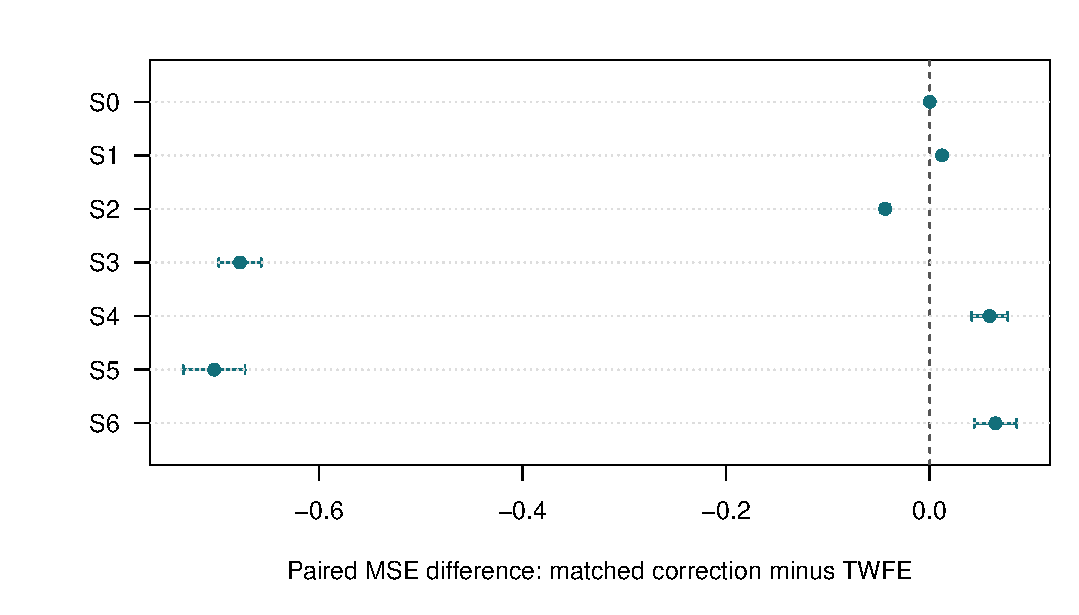
\includegraphics[width=0.92\linewidth]{figures/scenario_matched_paired_mse.pdf}
\caption{Paired mean squared error differences between the scenario-matched correction and TWFE. Negative values favor the correction. Bars show 1.96 Monte Carlo standard errors; they quantify simulation uncertainty and are not treatment-effect confidence intervals.}\label{fig:matchedpaired}
\end{figure}

\subsection{Updated six-estimator comparison}
The full comparison in Table~\ref{tab:overall} and Figure~\ref{fig:comparison} retains the original estimators and adds the scenario-matched benchmark. The matched estimator has the smallest absolute bias in S1--S6 and ties TWFE and the common-slope adjustment in S0. It has the lowest RMSE in S2, S3 and S5. In S1, S4 and S6, its near-zero bias comes with sufficient variance that TWFE or another original estimator has lower RMSE. The original common-slope adjustment remains exactly equal to TWFE in every replication; it should not be confused with the new group-gap regression, which permits the treated--control gap to evolve.

{\small\begin{longtable}{llrrrr}
\caption{Updated Monte Carlo performance across six estimators.}\label{tab:overall}\\
\toprule
Scenario & Estimator & Mean & Bias & RMSE & Variance \\
\midrule
\endfirsthead
\multicolumn{6}{l}{\textit{Table \ref{tab:overall} continued}}\\
\toprule
Scenario & Estimator & Mean & Bias & RMSE & Variance \\
\midrule
\endhead
\midrule
\multicolumn{6}{r}{\textit{Continued on next page}}\\
\endfoot
\bottomrule
\endlastfoot
S0 & Matched gap adj. & 1.9942 & -0.0058 & 0.0651 & 0.00421 \\
 & TWFE & 1.9942 & -0.0058 & 0.0651 & 0.00421 \\
 & Common-slope adj. & 1.9942 & -0.0058 & 0.0651 & 0.00421 \\
 & SC adj. & 1.9954 & -0.0046 & 0.0645 & 0.00413 \\
 & RF adj. & 1.9986 & -0.0014 & 0.0965 & 0.00930 \\
 & GBM adj. & 1.9966 & -0.0034 & 0.0787 & 0.00619 \\
\midrule
S1 & Matched gap adj. & 1.9965 & -0.0035 & 0.1372 & 0.01880 \\
 & TWFE & 2.0406 & 0.0406 & 0.0819 & 0.00505 \\
 & Common-slope adj. & 2.0406 & 0.0406 & 0.0819 & 0.00505 \\
 & SC adj. & 2.0413 & 0.0413 & 0.0822 & 0.00505 \\
 & RF adj. & 2.0273 & 0.0273 & 0.0988 & 0.00902 \\
 & GBM adj. & 2.0476 & 0.0476 & 0.1024 & 0.00823 \\
\midrule
S2 & Matched gap adj. & 2.0002 & 0.0002 & 0.1344 & 0.01805 \\
 & TWFE & 2.2280 & 0.2280 & 0.2486 & 0.00980 \\
 & Common-slope adj. & 2.2280 & 0.2280 & 0.2486 & 0.00980 \\
 & SC adj. & 2.2221 & 0.2221 & 0.2428 & 0.00964 \\
 & RF adj. & 2.1443 & 0.1443 & 0.1781 & 0.01090 \\
 & GBM adj. & 2.2522 & 0.2522 & 0.2736 & 0.01127 \\
\midrule
S3 & Matched gap adj. & 1.9955 & -0.0045 & 0.1377 & 0.01893 \\
 & TWFE & 2.8222 & 0.8222 & 0.8345 & 0.02032 \\
 & Common-slope adj. & 2.8222 & 0.8222 & 0.8345 & 0.02032 \\
 & SC adj. & 2.6914 & 0.6914 & 0.7089 & 0.02459 \\
 & RF adj. & 2.4942 & 0.4942 & 0.5088 & 0.01469 \\
 & GBM adj. & 2.6997 & 0.6997 & 0.7093 & 0.01343 \\
\midrule
S4 & Matched gap adj. & 1.9686 & -0.0314 & 0.3733 & 0.13836 \\
 & TWFE & 2.2647 & 0.2647 & 0.2836 & 0.01039 \\
 & Common-slope adj. & 2.2647 & 0.2647 & 0.2836 & 0.01039 \\
 & SC adj. & 2.2652 & 0.2652 & 0.2841 & 0.01040 \\
 & RF adj. & 2.1918 & 0.1918 & 0.2217 & 0.01235 \\
 & GBM adj. & 2.2747 & 0.2747 & 0.2972 & 0.01284 \\
\midrule
S5 & Matched gap adj. & 1.9977 & -0.0023 & 0.4058 & 0.16469 \\
 & TWFE & 2.9194 & 0.9194 & 0.9314 & 0.02214 \\
 & Common-slope adj. & 2.9194 & 0.9194 & 0.9314 & 0.02214 \\
 & SC adj. & 2.8927 & 0.8927 & 0.9054 & 0.02290 \\
 & RF adj. & 2.6692 & 0.6692 & 0.6827 & 0.01829 \\
 & GBM adj. & 2.8761 & 0.8761 & 0.8860 & 0.01741 \\
\midrule
S6 & Matched gap adj. & 2.0012 & 0.0012 & 0.3971 & 0.15772 \\
 & TWFE & 2.2295 & 0.2295 & 0.3052 & 0.04047 \\
 & Common-slope adj. & 2.2295 & 0.2295 & 0.3052 & 0.04047 \\
 & SC adj. & 2.2702 & 0.2702 & 0.3338 & 0.03844 \\
 & RF adj. & 2.1380 & 0.1380 & 0.3205 & 0.08367 \\
 & GBM adj. & 2.2472 & 0.2472 & 0.3184 & 0.04025 \\
\end{longtable}}

\begin{figure}[htbp]
\centering
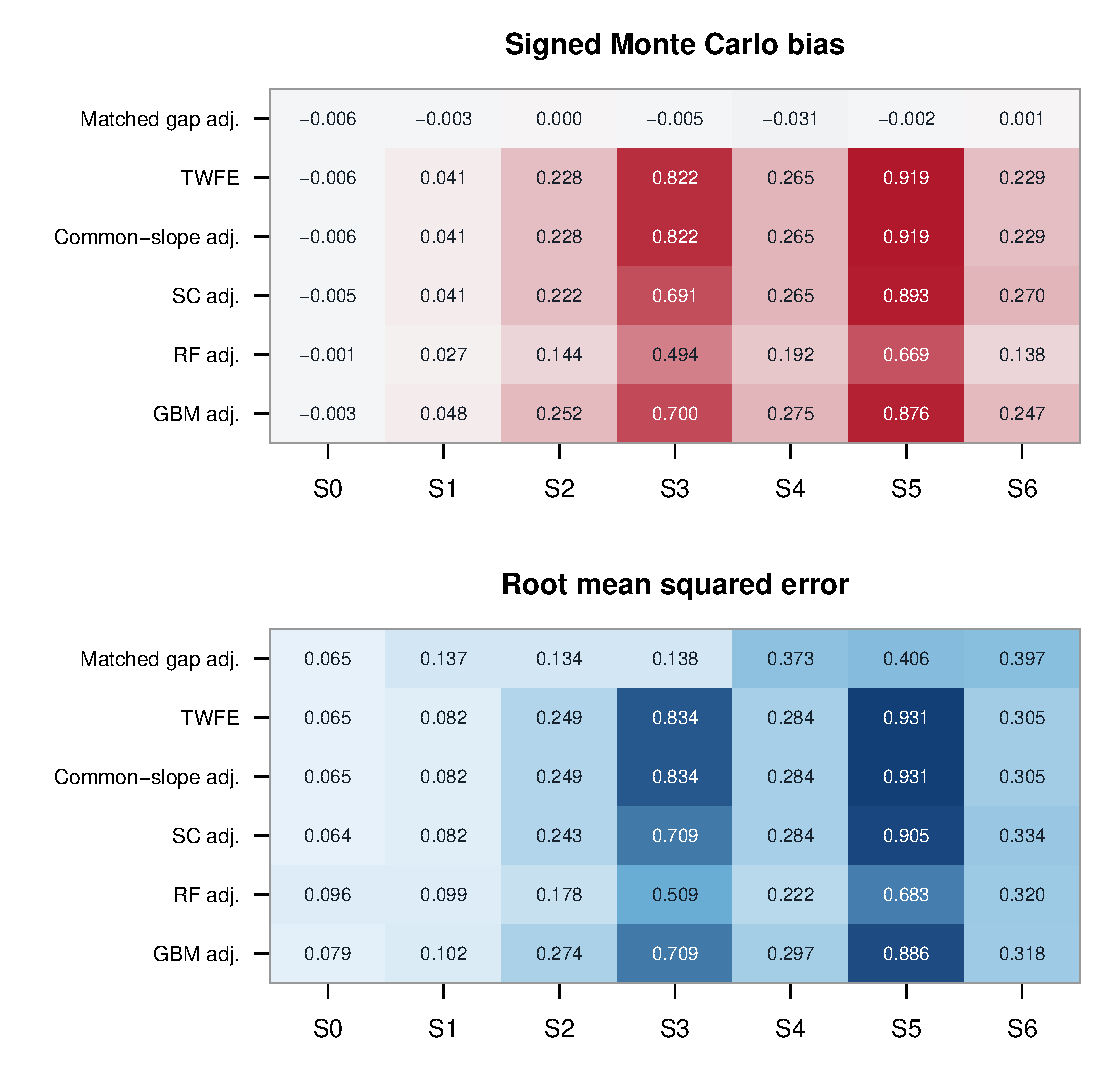
\includegraphics[width=0.94\linewidth]{figures/updated_bias_rmse_comparison.pdf}
\caption{Signed bias and RMSE for the scenario-matched benchmark, TWFE and the four original adjustments. Values use 500 replications per scenario.}\label{fig:comparison}
\end{figure}

\clearpage
\section{Evaluation}\label{sec:evaluation}
\subsection{What changes when the correction matches the violation}
The earlier common-slope model estimated one time slope shared by treated and control units. That slope cancels when group predictions are differenced, forcing the predicted gap to be constant and the estimated correction to zero. The new linear-gap procedure instead estimates the slope of the group difference itself. It can therefore recover a linear selection-bias path. For quadratic violations, the additional squared-time term is essential: a linear extrapolation would force constant growth in a gap whose slope is changing.

The near-zero average biases in S1--S6 show that this distinction matters. Under the simulated DGP, the untreated group gap is linear or quadratic apart from group-average disturbance noise, so the matched regression targets the same post-minus-pre gap change that contaminates TWFE. This is a statement about correct specification in this design. It does not show that a researcher can infer the true polynomial order from one short pre-treatment series without error.

\subsection{Bias--variance trade-off}
The matched correction estimates a small time series of group gaps and extrapolates beyond its observed support. Even with the correct order, coefficient noise is magnified by the post-treatment horizon. The linear correction has variance about 0.018--0.019 in S1--S3, compared with TWFE variance between 0.004 and 0.020. Its extra variance is worthwhile only once the linear violation is large enough. High outcome noise increases the matched estimator's variance to 0.1577 in S6. The quadratic correction is more variable because the linear and squared-time coefficients jointly determine predictions outside the training range; its variance is 0.1384 in S4 and 0.1647 in S5.

These results clarify the supervisor's point. Different violation shapes require different correction functions, but matching the shape addresses bias rather than guaranteeing lower RMSE. A useful correction must balance three features: whether the functional form is credible, whether the pre-period contains enough information to estimate it, and whether the violation is large enough to justify the added sampling variation.

\subsection{Relation to the original forecasting methods}
The original methods remain informative as deliberately imperfect alternatives. Synthetic Control matches one pre-treatment mean and need not reproduce a latent trend loading. Random Forest and Gradient Boosting use constant-leaf trees; with all post-treatment dates beyond the training support, their unit-level post-treatment forecasts are flat. Random Forest partially reduces bias in several scenarios, but it does not fully extrapolate continued linear or quadratic divergence. The matched polynomial benchmark isolates the gain available from imposing the correct functional form, while the comparison methods illustrate what happens when prediction flexibility within the pre-period does not translate into appropriate extrapolation.

The methods also use different information sets. Synthetic Control uses contemporaneous untreated donor outcomes after treatment, whereas the polynomial and other prediction models train on pre-treatment outcomes. The comparison should therefore be read as a comparison of complete procedures, not pure algorithms holding all inputs fixed.

\subsection{Limitations of the simulation study}
The simulation fixes the number of units, periods, treatment date, treatment effect and error structure. It excludes serial correlation, common shocks, staggered adoption, treatment-effect heterogeneity, missingness and structural breaks. Only twelve pre-treatment gap observations estimate each polynomial. Standard errors and confidence-interval coverage for the adjusted estimators are not developed here.

The main new limitation is explicit use of scenario labels to choose the correction. This is appropriate for an oracle simulation benchmark because it asks whether the right functional form can remove the designed violation. It would be invalid to present the same rule as an empirical estimator when the true counterfactual shape is unknown. The empirical study below therefore pre-specifies no correction, a linear group gap, Synthetic Control, Random Forest and Gradient Boosting, selects among them using rolling pre-treatment windows, and reports all five estimates as sensitivity results. Its machine-learning features differ from the simulated covariates because those covariates are not available in the homicide data.

Within these limits, the simulation supports a precise conclusion: scenario-matched gap extrapolation removes average selection bias, but it improves overall accuracy only when the avoided bias is large relative to extrapolation variance. This conclusion is stronger and more narrowly defined than a claim that one correction should be used for every violation scenario.

\clearpage
\section{Empirical Study}\label{sec:empirical}

\subsection{Institutional setting, source audit, and analysis sample}
The empirical application re-examines the 18 February--1 March 2020 police strike in Cear\'a studied by \cite{mancha2025}. The primary source is the 27,830 victim records in \texttt{Painel.xlsx}; \texttt{Gang\_Turfs.xlsx} supplies the gang-exposure measure. The released \texttt{Daily\_Homicides\_CE.dta} is an intermediate aggregation of the victim records, not independent evidence. We reconstruct its outcomes from the spreadsheet and compare unit--day totals after identical AIS and municipality normalization. The intermediate file has one duplicated unit--day; after re-aggregation its 27,418 valid-AIS homicides and all unit--day outcome counts agree with the source reconstruction. Seven exact duplicate source rows are retained because the data are victim records and the source does not establish that they are duplicate victims.

We exclude 412 records with absent or non-geographic AIS labels, retain 358 municipality/district units in 22 AIS, and balance every unit over 2,557 dates (1 January 2014--31 December 2020). Of 915,406 unit--days, 893,515 have no recorded homicide and are filled with zero. The main 97-day window has 34,726 unit--days (33,943 zero), 989 victim records, 94 treated units and 264 controls. The seven outcomes are total homicides, men, women, and the released \texttt{crime\_1}--\texttt{crime\_4} indicators, all as unit--day counts. To reproduce the released Stata coding, women equal total minus men; 24 records with unclassified sex therefore enter this residual category. This is a measurement limitation, not an assertion that their victims were female. The original spreadsheet, intermediate file, source-code hash, row flow, and discrepancy checks are preserved in the accompanying reproduction archive.

The primary treated set is AIS 02, 06, 11, 12, and 13, matching the paper's stated five high-exposure areas. The released Stata code lowercases AIS labels and later tests the uppercase literal \texttt{AIS 13}; that test fails, making its executed treated set AIS 02, 06, 11, and 12. We use this four-AIS version only as a replication and sensitivity case. A separate boundary issue arises from the 75th percentile of \texttt{ExposureDistricts}: its value is 0.587728, whereas AIS 07 is 0.588235. A mechanical ``greater than percentile'' rule includes AIS 07 and yields six areas. We report that six-AIS case separately rather than silently redefine the paper's intended five areas.

\subsection{Common TWFE benchmark and gap correction}
The analysis window consists of the 84 days ending 17 February 2020 and the 13 strike days. Each municipality/district receives equal weight within its treatment arm. The common benchmark is the coefficient on $D_i\times S_t$ in
\begin{equation}\label{eq:empiricaltwfe}
Y_{it}=\alpha_i+\lambda_t+\tau^{\mathrm{TWFE}}D_iS_t+u_{it},
\end{equation}
where $\alpha_i$ and $\lambda_t$ are unit and date effects. With the balanced panel and one common treatment date, direct two-way residualization verifies that this coefficient equals the post-strike treated-minus-control gap less the pre-strike mean gap for all seven outcomes; the largest numerical discrepancy is $6.8\times10^{-15}$.

Let $G_t$ denote that daily unit-weighted group gap. For each candidate $m$ we use the \emph{same} $\widehat\tau^{\mathrm{TWFE}}$ and pre-period baseline:
\begin{equation}\label{eq:empiricalbias}
\widehat B_m=\overline{\widehat G^{0}_{m,\mathrm{post}}}-\overline G_{\mathrm{pre}},\qquad
\widehat\tau_m=\widehat\tau^{\mathrm{TWFE}}-\widehat B_m
=\overline G_{\mathrm{post}}-\overline{\widehat G^{0}_{m,\mathrm{post}}}.
\end{equation}
Every forecast is averaged over seven days in the first strike block and six in the second, equivalently weighting the two block means by $7/13$ and $6/13$. The no-correction forecast sets $\overline{\widehat G^{0}}=\overline G_{\mathrm{pre}}$. The linear-gap method fits an ordinary line to twelve pre-strike weekly gap means and extrapolates weeks 13 and 14. Synthetic Control matches the treated arm's single 84-day pre-mean with nonnegative control-unit donor weights summing to one, then uses contemporaneous donor outcomes to forecast the treated mean and subtracts the contemporaneous unweighted control mean. Because a single matching predictor leaves many exact solutions, this implementation uses a maximum-entropy tie-break based on donor multiplicity; it is a transparent empirical implementation of the simulation's one-predictor design, not a claim to reproduce every numerical detail of the original \texttt{Synth} solver.

The Random Forest and Gradient Boosting retain the simulation's tree counts and major tuning choices (500 trees and two candidate features per forest split; 800 depth-three boosting trees, learning rate 0.01, leaf size ten, subsample 0.7). Their empirical prediction target is different. The simulated $X_1,X_2,X_3$ do not exist in these data, so each model fits the two daily \emph{group mean} series, using only relative day, treatment-arm label, weekday and calendar month. It predicts both group means and takes their difference. Relative day, weekday, month, and arm label are known at forecast time. Models are refitted inside each window. Synthetic Control may use contemporaneous control outcomes; no candidate uses strike-period treated outcomes to fit or select its counterfactual. Forest and boosting forecasts beyond the training dates should not be interpreted as unrestricted extrapolation of a latent trend: terminal-tree predictions are bounded by training responses.

\subsection{Pre-strike evaluation and selection}
The true untreated strike-period gap is unobserved, so empirical ATT bias cannot be measured. We instead run the same 84-day training/13-day testing exercise at 154 pre-strike origins, moving the origin by 14 days each time. Each origin re-estimates all five candidates and treats the ensuing 13 days as a zero-effect placebo. The resulting pseudo-effect is $\overline G_{\mathrm{test}}-\overline{\widehat G^0_{m,\mathrm{test}}}$, algebraically the common placebo TWFE less the candidate's predicted bias term. We report mean signed error, population variance, MAE, RMSE, available windows, and failures. The winner for each outcome is fixed by the smallest pre-strike placebo RMSE, with no inspection of strike outcomes. The 13-day test blocks do not overlap at a 14-day step, but adjacent 84-day training blocks do; paired window differences are correlated and a naive window-level standard error is not an independent-sample uncertainty measure.

\begin{table}[htbp]
\centering\small
\caption{Total-homicide rolling pre-strike placebo performance (154 windows, 84-day training and 13-day test). The pseudo-effect is zero; variance is the population variance of placebo estimates. SC--entropy uses an entropy tie-break; RF--empirical and GB--empirical use forecast-known calendar and group features.}
\label{tab:placeborebuild}
\begin{tabular}{lrrrrrr}
\toprule
Method & Signed error & Variance & MAE & RMSE & Windows & Failures\\
\midrule
No correction & 0.00028 & 0.000069 & 0.00675 & 0.00830 & 154 & 0\\
Linear gap & -0.00008 & 0.000090 & 0.00755 & 0.00946 & 154 & 0\\
SC--entropy & 0.00105 & 0.000076 & 0.00718 & 0.00876 & 154 & 0\\
RF--empirical & 0.00202 & 0.000061 & 0.00642 & 0.00809 & 154 & 0\\
GB--empirical & 0.00018 & 0.000067 & 0.00655 & 0.00820 & 154 & 0\\
\bottomrule
\end{tabular}
\end{table}


For total homicides, Random Forest has the smallest pre-strike RMSE (0.00809), versus 0.00830 for no correction, 0.00820 for Gradient Boosting, 0.00876 for Synthetic Control, and 0.00946 for the linear gap. Its 2.6\% advantage over unadjusted TWFE is modest, and it has a positive mean signed placebo error (0.00202), so this ranking is evidence of relative pre-period prediction, not proof that strike-period selection bias was eliminated. A lag-six HAC sensitivity for the paired forest-versus-TWFE MSE difference gives $-3.49\times10^{-6}$ with a standard error of $6.42\times10^{-6}$; it does not resolve the close ranking statistically. Random Forest also ranks first for men, women and three of the four crime indicators; no correction ranks first for \texttt{crime\_4}. The full all-outcome performance table is in Table~\ref{tab:allplaceborebuild} below.

\begin{figure}[htbp]\centering
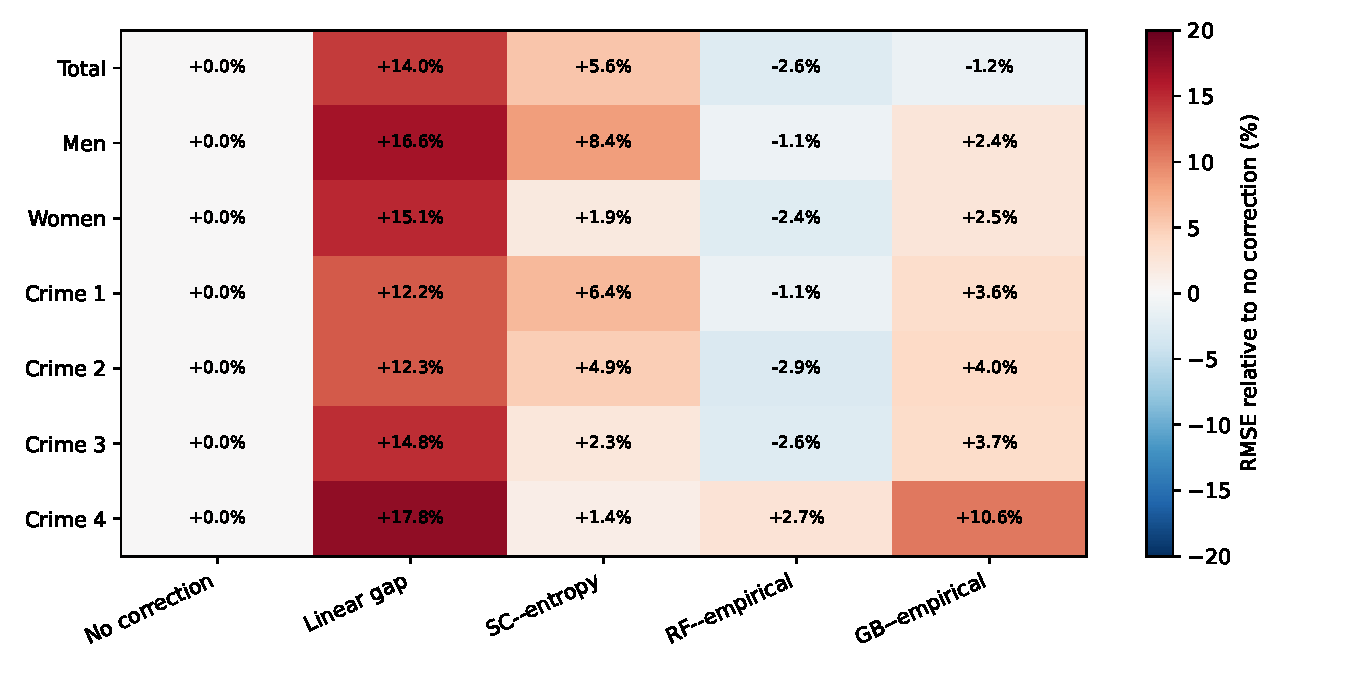
\includegraphics[width=0.88\linewidth]{figures/empirical_rmse_rebuild.pdf}
\caption{Pre-strike placebo RMSE relative to no correction; negative values indicate lower RMSE. All comparisons use the same 154 rolling windows.}\label{fig:empiricalrmserebuild}
\end{figure}

\subsection{Strike-period estimates and AIS resampling}
After the selection rule is frozen, all five methods are refitted on the actual 84 pre-strike days, and every pre-specified estimate is reported. For total homicides the common TWFE DID is 0.03437 per municipality/district-day. The linear, Synthetic Control, Random Forest, and Gradient Boosting predicted bias terms are respectively 0.00732, 0.04560, $-0.00169$, and $-0.00136$, giving adjusted estimates 0.02705, $-0.01123$, 0.03606, and 0.03573. Synthetic Control's larger downward adjustment reflects its donor-based forecast of a higher untreated strike-period gap; its information set differs because the control outcomes are contemporaneous. It was not selected by the pre-strike rule. Table~\ref{tab:estimatesrebuild} gives every outcome, the identical within-outcome TWFE, its candidate-specific bias term, corrected estimate and fixed-method interval.

\begin{longtable}{llrrrrl}
\caption{Strike-period TWFE, predicted bias and correction on the common unit/date panel. Percentile intervals resample AIS within treatment arms; * marks the pre-strike RMSE winner.}\label{tab:estimatesrebuild}\\
\toprule
Outcome & Method & TWFE & Bias $\widehat B_m$ & Adjusted & 95\% interval & Selected\\
\midrule
\endfirsthead
\toprule
Outcome & Method & TWFE & Bias & Adjusted & 95\% interval & Selected\\
\midrule
\endhead
Total & No correction & 0.0344 & 0.0000 & 0.0344 & [-0.016, 0.142] & \\
Total & Linear gap & 0.0344 & 0.0073 & 0.0271 & [-0.018, 0.135] & \\
Total & SC--entropy & 0.0344 & 0.0456 & -0.0112 & [-0.045, 0.065] & \\
Total & RF--empirical & 0.0344 & -0.0017 & 0.0361 & [-0.013, 0.155] & *\\
Total & GB--empirical & 0.0344 & -0.0014 & 0.0357 & [-0.012, 0.156] & \\
\midrule
Men & No correction & 0.0320 & 0.0000 & 0.0320 & [-0.015, 0.144] & \\
Men & Linear gap & 0.0320 & 0.0062 & 0.0257 & [-0.017, 0.135] & \\
Men & SC--entropy & 0.0320 & 0.0416 & -0.0096 & [-0.039, 0.067] & \\
Men & RF--empirical & 0.0320 & -0.0045 & 0.0365 & [-0.008, 0.152] & *\\
Men & GB--empirical & 0.0320 & -0.0052 & 0.0372 & [-0.007, 0.153] & \\
\midrule
Women & No correction & 0.0024 & 0.0000 & 0.0024 & [-0.007, 0.011] & \\
Women & Linear gap & 0.0024 & 0.0011 & 0.0013 & [-0.009, 0.011] & \\
Women & SC--entropy & 0.0024 & -0.0012 & 0.0036 & [-0.008, 0.012] & \\
Women & RF--empirical & 0.0024 & 0.0008 & 0.0016 & [-0.007, 0.012] & *\\
Women & GB--empirical & 0.0024 & 0.0027 & -0.0003 & [-0.010, 0.010] & \\
\midrule
Crime 1 & No correction & 0.0214 & 0.0000 & 0.0214 & [-0.006, 0.076] & \\
Crime 1 & Linear gap & 0.0214 & 0.0020 & 0.0195 & [-0.007, 0.075] & \\
Crime 1 & SC--entropy & 0.0214 & 0.0186 & 0.0028 & [-0.020, 0.051] & \\
Crime 1 & RF--empirical & 0.0214 & -0.0048 & 0.0262 & [-0.002, 0.081] & *\\
Crime 1 & GB--empirical & 0.0214 & -0.0044 & 0.0258 & [-0.002, 0.082] & \\
\midrule
Crime 2 & No correction & 0.0178 & 0.0000 & 0.0178 & [-0.008, 0.067] & \\
Crime 2 & Linear gap & 0.0178 & 0.0026 & 0.0152 & [-0.009, 0.064] & \\
Crime 2 & SC--entropy & 0.0178 & 0.0163 & 0.0015 & [-0.021, 0.045] & \\
Crime 2 & RF--empirical & 0.0178 & -0.0031 & 0.0209 & [-0.005, 0.070] & *\\
Crime 2 & GB--empirical & 0.0178 & -0.0026 & 0.0205 & [-0.004, 0.069] & \\
\midrule
Crime 3 & No correction & 0.0120 & 0.0000 & 0.0120 & [-0.010, 0.051] & \\
Crime 3 & Linear gap & 0.0120 & 0.0032 & 0.0088 & [-0.013, 0.044] & \\
Crime 3 & SC--entropy & 0.0120 & 0.0122 & -0.0002 & [-0.022, 0.034] & \\
Crime 3 & RF--empirical & 0.0120 & -0.0024 & 0.0144 & [-0.006, 0.051] & *\\
Crime 3 & GB--empirical & 0.0120 & -0.0028 & 0.0148 & [-0.005, 0.052] & \\
\midrule
Crime 4 & No correction & 0.0094 & 0.0000 & 0.0094 & [-0.012, 0.047] & *\\
Crime 4 & Linear gap & 0.0094 & 0.0030 & 0.0063 & [-0.015, 0.046] & \\
Crime 4 & SC--entropy & 0.0094 & 0.0094 & -0.0000 & [-0.021, 0.038] & \\
Crime 4 & RF--empirical & 0.0094 & -0.0016 & 0.0110 & [-0.010, 0.050] & \\
Crime 4 & GB--empirical & 0.0094 & -0.0014 & 0.0108 & [-0.010, 0.049] & \\
\bottomrule
\end{longtable}


For fixed-method uncertainty we resample AIS, with replacement separately among five treated and seventeen control clusters, and refit the final 84/13-day calculation on each draw. Percentile intervals summarize 499 draws for each of 35 outcome--method estimates. The selected total-homicide Random Forest interval is $[-0.0126,0.1552]$, and none of the seven selected fixed-method intervals excludes zero. For total homicides we additionally repeat the \emph{entire} 154-window model-selection exercise inside each of 99 AIS draws, then refit that draw's selected method in the strike window. The re-selection result is reported separately from fixed-method intervals. Only five treated AIS are available, so neither percentile construction nor model re-selection removes substantial few-cluster uncertainty; the 99-draw selection-aware interval in particular has coarse tail resolution. AIS resampling also assumes that these clusters are a meaningful basis for uncertainty, not that treatment is randomized across them.

\begin{table}[htbp]
\centering\small
\caption{Fixed-method versus full selection-aware AIS bootstrap for total homicides. Both rows share the original-sample point estimate; percentile intervals differ in whether selection is repeated.}
\label{tab:selectionrebuild}
\begin{tabular}{lrrrl}
\toprule
Procedure & Draws & Estimate & 95\% interval & Re-selection\\
\midrule
Random Forest fixed & 499 & 0.0361 & [-0.0126, 0.1552] & No\\
Full RMSE selection & 99 & 0.0361 & [-0.0254, 0.1433] & Yes\\
\bottomrule
\end{tabular}
\end{table}

Across 99 selection-aware resamples, the pre-strike RMSE rule chose no correction 61, linear gap 0, Synthetic Control 19, Random Forest 15, Gradient Boosting 4. The observed-sample winner was Random Forest. Selection changes across draws, showing that the small placebo-RMSE advantage is sensitive to AIS composition. Neither interval is a randomization-based causal interval.


\begin{figure}[htbp]\centering
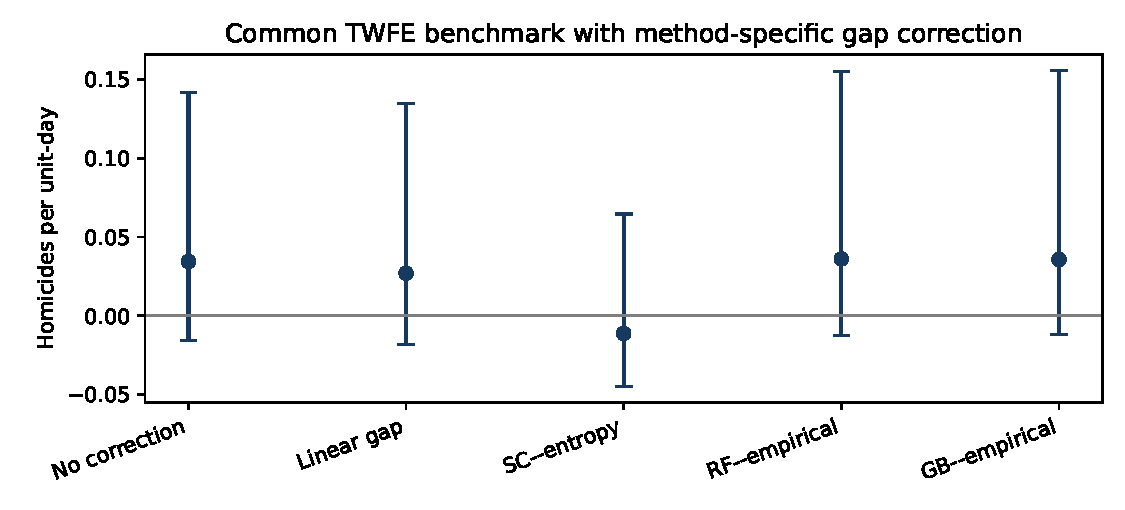
\includegraphics[width=0.82\linewidth]{figures/empirical_total_estimates_rebuild.pdf}
\caption{Total-homicide estimates and fixed-method 95\% AIS-bootstrap percentile intervals, all aligned to the same TWFE benchmark. The displayed intervals do not repeat model selection; Table~\ref{tab:selectionrebuild} gives the selection-aware comparison.}\label{fig:totalestimatesrebuild}
\end{figure}

\begin{figure}[htbp]\centering
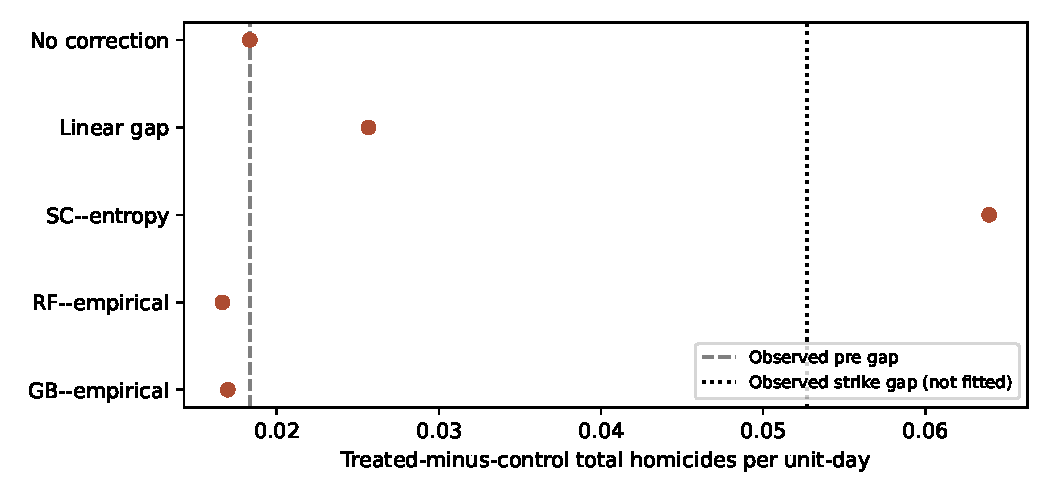
\includegraphics[width=0.83\linewidth]{figures/empirical_counterfactual_gap_rebuild.pdf}
\caption{Total-homicide untreated strike-gap forecasts. The observed strike gap is displayed only for comparison and is excluded from every candidate's fit and from the pre-strike selection.}\label{fig:counterfactualrebuild}
\end{figure}

\subsection{External comparison and sensitivity}
The released Mancha specification regresses the nonzero-observation unit--day outcome on a statewide strike indicator and its interaction with high gang exposure, absorbing municipality/district, AIS--year, month and weekday effects. It uses the 2014--2020 source sample rather than the balanced 97-day main window; in our replication it has 21,886 source unit--day observations after the original singleton/duplicate handling. Its interaction is not the unit/date TWFE DID in Equation~\ref{eq:empiricaltwfe}: zero-filled days, date effects, sample duration, implicit observation weights and, for the published code, treatment coding all differ. With the executed four-AIS coding, the reproduced total-homicide interaction is 0.334996, matching the published 0.335 after rounding. Six other reproduced interactions are within 0.0006 of the printed coefficients; the largest discrepancy is for women (0.068401 versus published 0.069), which is not identical at three-decimal rounding and remains unresolved. Correcting that \emph{same} external specification to five AIS gives 0.224398. Neither coefficient is inserted into Equation~\ref{eq:empiricalbias}; the difference from this thesis's 0.03437 TWFE is not an estimate of ``bias corrected away.''

\begin{table}[htbp]
\centering\small
\caption{External replication of Mancha's interaction regression versus this thesis's distinct TWFE benchmark. Coefficients are not subtracted from one another.}
\label{tab:mancharebuild}
\begin{tabular}{lrrrr}
\toprule
Outcome & Published & Replicated four AIS & Corrected five AIS & Thesis TWFE\\
\midrule
Total & 0.335 & 0.335 & 0.224 & 0.034\\
Men & 0.267 & 0.267 & 0.184 & 0.032\\
Women & 0.069 & 0.068 & 0.040 & 0.002\\
Crime 1 & 0.297 & 0.297 & 0.236 & 0.021\\
Crime 2 & 0.267 & 0.267 & 0.188 & 0.018\\
Crime 3 & 0.180 & 0.180 & 0.083 & 0.012\\
Crime 4 & 0.159 & 0.159 & 0.060 & 0.009\\
\bottomrule
\end{tabular}
\end{table}


Table~\ref{tab:sensitivityrebuild} changes the pre-period from 8 to 104 weeks, applies the executed four-AIS and mechanical six-AIS definitions, and aggregates at AIS--day rather than municipality/district--day. Four-AIS coding increases the 12-week TWFE to about 0.0568; adding AIS 07 produces about 0.0349. The AIS aggregate estimates are on a different count scale and weight AIS equally instead of municipalities. Synthetic Control's negative main-window result is sensitive to horizon, becoming slightly positive at 104 weeks. These contrasts show that treatment definition, forecast support and analysis unit matter; they are not alternative measurements of a known ATT.

\begin{longtable}{lrrrrr}
\caption{Total-homicide sensitivity to pre-period length, treatment definition, and aggregation. Entries are adjusted estimates, not comparable across the last unit-aggregation row in absolute scale.}\label{tab:sensitivityrebuild}\\
\toprule
Specification & TWFE & Linear & SC & RF & GB\\
\midrule
Five AIS, 8 weeks & 0.032 & 0.027 & -0.011 & 0.037 & 0.036\\
Five AIS, 12 weeks & 0.034 & 0.027 & -0.011 & 0.036 & 0.036\\
Five AIS, 26 weeks & 0.037 & 0.031 & -0.011 & 0.036 & 0.036\\
Five AIS, 52 weeks & 0.038 & 0.036 & -0.011 & 0.035 & 0.036\\
Five AIS, 104 weeks & 0.037 & 0.038 & 0.003 & 0.035 & 0.034\\
Four AIS, 12 weeks & 0.057 & 0.050 & 0.008 & 0.061 & 0.061\\
Six AIS, 12 weeks & 0.035 & 0.029 & -0.019 & 0.038 & 0.037\\
AIS--day, 12 weeks & 0.767 & 0.619 & -0.754 & 0.790 & 0.785\\
\bottomrule
\end{longtable}


{\footnotesize\begin{longtable}{llrrrrrr}
\caption{All-outcome pre-strike placebo performance (same 154 windows and models in each row).}\label{tab:allplaceborebuild}\\
\toprule
Outcome & Method & Signed error & Variance & MAE & RMSE & Windows & Failures\\
\midrule
\endfirsthead
\toprule
Outcome & Method & Signed error & Variance & MAE & RMSE & Windows & Failures\\
\midrule
\endhead
Total & No correction & 0.00028 & 0.000069 & 0.00675 & 0.00830 & 154 & 0\\
Total & Linear gap & -0.00008 & 0.000090 & 0.00755 & 0.00946 & 154 & 0\\
Total & SC--entropy & 0.00105 & 0.000076 & 0.00718 & 0.00876 & 154 & 0\\
Total & RF--empirical & 0.00202 & 0.000061 & 0.00642 & 0.00809 & 154 & 0\\
Total & GB--empirical & 0.00018 & 0.000067 & 0.00655 & 0.00820 & 154 & 0\\
\midrule
Men & No correction & 0.00027 & 0.000060 & 0.00630 & 0.00775 & 154 & 0\\
Men & Linear gap & -0.00005 & 0.000082 & 0.00703 & 0.00904 & 154 & 0\\
Men & SC--entropy & 0.00102 & 0.000069 & 0.00682 & 0.00840 & 154 & 0\\
Men & RF--empirical & 0.00183 & 0.000055 & 0.00597 & 0.00767 & 154 & 0\\
Men & GB--empirical & 0.00020 & 0.000063 & 0.00620 & 0.00793 & 154 & 0\\
\midrule
Women & No correction & 0.00001 & 0.000004 & 0.00140 & 0.00188 & 154 & 0\\
Women & Linear gap & -0.00003 & 0.000005 & 0.00171 & 0.00216 & 154 & 0\\
Women & SC--entropy & 0.00034 & 0.000004 & 0.00148 & 0.00191 & 154 & 0\\
Women & RF--empirical & 0.00033 & 0.000003 & 0.00138 & 0.00183 & 154 & 0\\
Women & GB--empirical & 0.00004 & 0.000004 & 0.00154 & 0.00192 & 154 & 0\\
\midrule
Crime 1 & No correction & 0.00006 & 0.000030 & 0.00446 & 0.00544 & 154 & 0\\
Crime 1 & Linear gap & -0.00016 & 0.000037 & 0.00479 & 0.00610 & 154 & 0\\
Crime 1 & SC--entropy & 0.00057 & 0.000033 & 0.00463 & 0.00579 & 154 & 0\\
Crime 1 & RF--empirical & 0.00102 & 0.000028 & 0.00433 & 0.00538 & 154 & 0\\
Crime 1 & GB--empirical & 0.00003 & 0.000032 & 0.00450 & 0.00563 & 154 & 0\\
\midrule
Crime 2 & No correction & 0.00006 & 0.000025 & 0.00411 & 0.00497 & 154 & 0\\
Crime 2 & Linear gap & -0.00015 & 0.000031 & 0.00439 & 0.00559 & 154 & 0\\
Crime 2 & SC--entropy & 0.00056 & 0.000027 & 0.00423 & 0.00522 & 154 & 0\\
Crime 2 & RF--empirical & 0.00098 & 0.000022 & 0.00394 & 0.00483 & 154 & 0\\
Crime 2 & GB--empirical & 0.00007 & 0.000027 & 0.00413 & 0.00517 & 154 & 0\\
\midrule
Crime 3 & No correction & 0.00006 & 0.000019 & 0.00352 & 0.00439 & 154 & 0\\
Crime 3 & Linear gap & -0.00014 & 0.000025 & 0.00406 & 0.00504 & 154 & 0\\
Crime 3 & SC--entropy & 0.00056 & 0.000020 & 0.00357 & 0.00449 & 154 & 0\\
Crime 3 & RF--empirical & 0.00086 & 0.000018 & 0.00337 & 0.00428 & 154 & 0\\
Crime 3 & GB--empirical & 0.00003 & 0.000021 & 0.00363 & 0.00455 & 154 & 0\\
\midrule
Crime 4 & No correction & 0.00008 & 0.000016 & 0.00318 & 0.00402 & 154 & 0\\
Crime 4 & Linear gap & -0.00005 & 0.000022 & 0.00378 & 0.00474 & 154 & 0\\
Crime 4 & SC--entropy & 0.00056 & 0.000016 & 0.00324 & 0.00408 & 154 & 0\\
Crime 4 & RF--empirical & 0.00084 & 0.000016 & 0.00325 & 0.00413 & 154 & 0\\
Crime 4 & GB--empirical & 0.00011 & 0.000020 & 0.00350 & 0.00445 & 154 & 0\\
\bottomrule
\end{longtable}
}

\section{Discussion}\label{sec:discussion}
The simulation isolates the correction's mechanism: when the untreated gap's functional form is known, a matching forecast can largely remove its induced DID bias. Yet reducing signed bias can increase variance, so RMSE improves only when the avoided bias is large relative to extrapolation noise. That is an oracle result because the simulation knows the true functional form and ATT. The empirical study cannot observe either and therefore substitutes pre-strike out-of-sample pseudo-effects for model selection, not for direct estimation of true ATT bias.

The expanded Cear\'a comparison demonstrates why that distinction matters. The forest's slight pre-strike RMSE advantage selects it for total homicides in the original sample, but its strike adjustment is small and in the opposite direction from the linear and Synthetic Control adjustments. The full re-selection bootstrap instead chooses no correction in 61 of 99 draws and the forest in only 15, with Synthetic Control in 19 and boosting in four. This is direct evidence that the narrow pre-strike ranking is sensitive to AIS composition, not evidence about the unobserved strike counterfactual. The five candidates share one TWFE baseline and the same unit weights; differences arise from their forecasts of the missing untreated gap, not from substituting a published coefficient. The forest's win is not a universal algorithm ranking: its covariates had to be redefined because simulated $X_1,X_2,X_3$ were unavailable. Synthetic Control's use of contemporaneous donor outcomes is a different, potentially valuable information set, but the one-predictor matching design does not guarantee a credible post-strike untreated path.

Rolling placebo performance provides a disciplined comparison under historical no-treatment conditions. It does not establish that an unobserved untreated gap during a police strike would continue to obey the same relationship. Nor should overlapping training windows be interpreted as 154 independent experiments. The AIS bootstrap and selection-aware re-estimation address sampling and model-selection variation within the observed cluster structure, but five treated clusters leave wide scope for finite-cluster error and sensitivity to the composition of the treated arm. Sex classification, the ambiguous AIS 07 cutoff, and differences between the published and executed treatment code are additional measurement and design constraints.

The practical lesson is to state the estimating object before attempting a correction, align every forecast to its pre-period baseline and weights, pre-specify a no-correction candidate, select only with untreated pre-period evidence, and report the whole candidate set together with external estimands clearly separated. Such a workflow permits an adjustment without pretending that predictive validation identifies a missing causal counterfactual. Further work could compare longer-horizon validation, regularized forecasts, and inference designed specifically for very few treated clusters.

\section{Conclusion}\label{sec:conclusion}
This thesis evaluates a transparent DID bias correction: predict the untreated treated--control gap during treatment, subtract its change from the same pre-treatment gap embedded in TWFE, and keep that benchmark common to all methods. In the controlled simulation, a correctly specified correction can nearly eliminate average bias, but lower RMSE is conditional on a sufficiently strong violation. In the Cear\'a application, the original-sample pre-strike RMSE rule selects Random Forest for total homicides and five other outcomes, while retaining unadjusted TWFE for one. The selected total-homicide point estimate is close to TWFE, its pre-strike RMSE improvement is modest, and complete AIS resampling often selects a different method. The selected-procedure total-homicide interval includes zero. The substantive conclusion must therefore remain cautious: these calculations compare historically predictive counterfactual procedures, not directly observed strike-period ATT bias. The value of the framework is its auditable link between estimand, forecast, validation, uncertainty and sensitivity, rather than a claim that one adjustment always dominates.


\begin{thebibliography}{9}
\bibitem{mancha2025}
Mancha, A. (2025).
When the State steps down: Reduced police surveillance and gang-related deaths in Brazil.
\emph{World Development}, 189, 106925.
\end{thebibliography}

\end{document}

